\documentclass[a4paper,12pt]{article} % тип документа

% report, book

% Рисунки
\usepackage{graphicx}
\usepackage{wrapfig}
\usepackage{mathtext}
\usepackage[left=2cm,right=2cm,
    top=2cm,bottom=2cm,bindingoffset=0cm]{geometry}

\usepackage{hyperref}
\usepackage[rgb]{xcolor}
\hypersetup{				% Гиперссылки
    colorlinks=true,       	% false: ссылки в рамках
	urlcolor=blue          % на URL
}

%  Русский язык

\usepackage[T2A]{fontenc}			% кодировка
\usepackage[utf8]{inputenc}			% кодировка исходного текста
\usepackage[english,russian]{babel}	% локализация и переносы


% Математика
\usepackage{amsmath,amsfonts,amssymb,amsthm,mathtools} 


\usepackage{wasysym}

\author{Анна Назарчук Б02-109}
\title{2.5.1 Измерение коэффициента поверхностного натяжения жидкости}
\date{}
\begin{document}
\maketitle
\section{Аннотация}
В работе исследуется коэффициент поверхностного натяжения воды и его температурная зависимость с помощью прибора Ребиндера.

\textbf{Цель:} 1. измерение температурной зависимости  коэффициента поверхностного натяжения дистиллированной воды с использованием известного коэффициента поверхностного натяжения спирта;  2. определение полной поверхностной энергии  и теплоты, необходимой для изотермического образования единицы  поверхности жидкости  при различной температуре. 

\textbf{Оборудование:}прибор  Ребиндера  с термостатом и микроманометром; исследуемые жидкости; стаканы.

\section{Теоретические сведения}
Из-за поверхностного натяжения возникают разные далвения с разных сторон искривленной поверхности жидкости:
\begin{equation}
\Delta P = P_{внутри} - P_{снаружи} = \frac{2\sigma}{r} \;(формула\; Лапласа)
\end{equation}
$\sigma$ - коэффицент поверхностного натяжения, $r$ - радиус кривизны поверхности.

\section{Экспериментальная установка и методика измерений}
\begin{figure}[h!]
\begin{center}
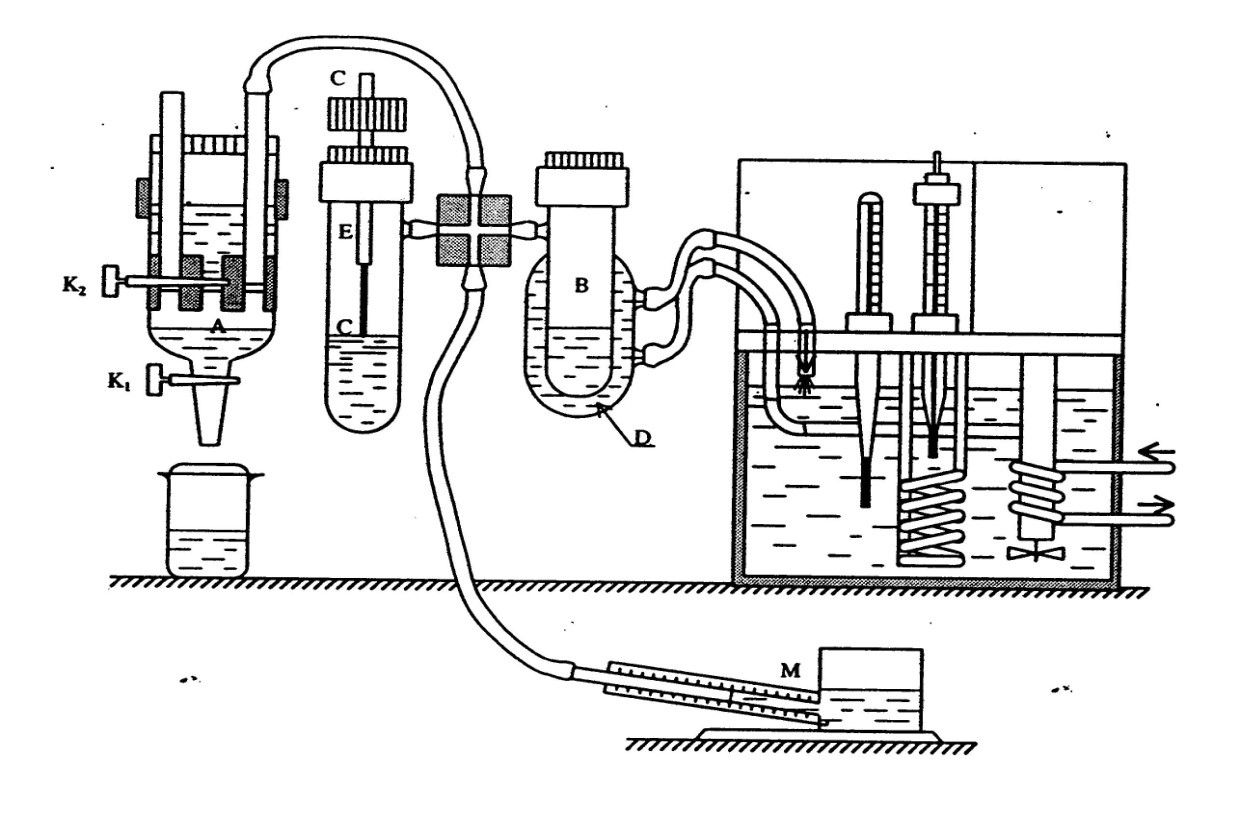
\includegraphics[width=\textwidth]{Установка}
\end{center}
\caption{Схема установки} \label{установка}
\end{figure}
Схема экспериментальной установки представлена на рисунке \ref{установка}.
Тестовая жидкость (этиловый спирт) наливается в сосуд, через пробку в него входит полая металлическа игла. При создании достаточно разреженного воздуха в колбе пузырьки воздуха начинают пробулькивать, поверхностное натяжение измеряется по величине разряжения. Разряжение создается с помощью аспиратора, разность давлений измеряется спиртовым микроманометром.

Для стабилизации температуры через рубашку колбы с исследуемой жидкостью прогоняется вода из термостата. Из-за большой теплопроводности трубки температура в разных частях трубки заметно различна и ввиду теплового расширения поднимается уровень жидкости при изменении температуры. Поэтому при температурном измерениии кончик иглы опускают до самого дна сосуда, тогда:
\begin{equation}
\Delta P = P - \rho g h
\end{equation}
$\rho$ - плотность жидкости, $h$ - высота погружения иглы.

\section{Измерения и обработка данных}
\subsection*{Измерение радиуса иглы}
Измерение радиусы иглы проводится двумя различными способами: с помощью коэффиента поверхностного натяжения спирта и непосредственно на микроскопе.
 
\begin{table}[h!]
\caption{Показания микроманометра при измерениях на спирте}
\label{спирт}
\begin{tabular}{|l|l|l|l|l|l|l|l|l|}
\hline
h & 35 & 35 & 35 & 35 & 35 & 35.5 & 35.5 & 35.5 \\ \hline
\end{tabular}
\end{table}
Данные показаний на спирте в таблице \ref{спирт}. Из них получается значение радиуса иглы (табл. \ref{радуис_спирт})
\begin{table}[h!]
\caption{Радуис иглы, измеренный через эталонную жидкость}
\label{радуис_спирт}
\begin{tabular}{|l|l|l|}
\hline
r, $10^{-3}$ м & $\sigma_r$,  $10^{-3}$м & $\varepsilon$, \% \\ \hline
0.66           & 0.007                   & 1.1            \\ \hline
\end{tabular}
\end{table}

При измерении на микроскопе получается радиус иглы, равный:
\begin{equation}
r = (0.6 \pm 0.003 )\cdot  10^{-3} \; м
\end{equation}
В дальнейшем примем $r$, равный измеренному на эталонной жидкости, так как рехультаты измерений близки друг к другу.
\subsection*{Измерения глубины погружения}
Сравним измеренную с помощью линейки высоту погружения с результами при погружении иглы в воду при комнатной температуре. 
Из первых двух столбцов таблицы с данными (\ref{данные}) получим и данных линейки, что:
\begin{table}[h!]
\caption{Высота погружения}
\label{высота}
\begin{tabular}{|l|l|l|l|}
\hline
$h_{\Delta P}$, $10^{-3}$ м & $\sigma_h$,  $10^{-3}$м & $\varepsilon$, \% & $h_{линейка}$ $10^{-3}$ м\\ \hline
6.27          & 0.13                   & 2.07    &    6     \\ \hline
\end{tabular}
\end{table}
\subsection*{Измерения коэффициента поверхностного натяжения воды при разных температурах}
Результаты измерений представлены в таблице \ref{данные}.

\begin{table}[h!]
\caption{Показания микроманометра при расположении иглы на глубине и поверхности при разных температурах}
\label{данные}
\begin{tabular}{|ll|ll|ll|ll|}
\hline
\multicolumn{2}{|l|}{t = 23 $^\circ$ C}            & \multicolumn{2}{l|}{t = 30 $^\circ$ C}            & \multicolumn{2}{l|}{t = 35 $^\circ$ C}            & \multicolumn{2}{l|}{t = 40 $^\circ$ C}            \\ \hline
\multicolumn{1}{|l|}{$h_{глубина}$} & $h_{пов-ть}$ & \multicolumn{1}{l|}{$h_{глубина}$} & $h_{пов-ть}$ & \multicolumn{1}{l|}{$h_{глубина}$} & $h_{пов-ть}$ & \multicolumn{1}{l|}{$h_{глубина}$} & $h_{пов-ть}$ \\ \hline
\multicolumn{1}{|l|}{144}           & 111.5        & \multicolumn{1}{l|}{141}           & 107.5        & \multicolumn{1}{l|}{138.5}         & 107.5        & \multicolumn{1}{l|}{137.5}         & 107          \\ \hline
\multicolumn{1}{|l|}{143.5}         & 110.5        & \multicolumn{1}{l|}{141}           & 107.5        & \multicolumn{1}{l|}{138.5}         & 107.5        & \multicolumn{1}{l|}{137.5}         & 107          \\ \hline
\multicolumn{1}{|l|}{143.5}         & 111          & \multicolumn{1}{l|}{141}           & 107.5        & \multicolumn{1}{l|}{138.5}         & 107.5        & \multicolumn{1}{l|}{137.5}         & 107          \\ \hline
\multicolumn{1}{|l|}{144}           & 111.5        & \multicolumn{1}{l|}{140.5}         & 107.5        & \multicolumn{1}{l|}{138.5}         & 107.5        & \multicolumn{1}{l|}{137.5}         & 107          \\ \hline
\multicolumn{1}{|l|}{143.5}         & 110.5        & \multicolumn{1}{l|}{140.5}         & 107.5        & \multicolumn{1}{l|}{138.5}         & 107.5        & \multicolumn{1}{l|}{137.5}         & 106.5        \\ \hline
\multicolumn{1}{|l|}{144}           & 110.5        & \multicolumn{1}{l|}{140.5}         & 107.5        & \multicolumn{1}{l|}{138.5}         & 107.5        & \multicolumn{1}{l|}{137}           & 106.5        \\ \hline
\multicolumn{1}{|l|}{143.5}         & 110.5        & \multicolumn{1}{l|}{140.5}         & 108          & \multicolumn{1}{l|}{138.5}         & 107.5        & \multicolumn{1}{l|}{137}           & 106.5        \\ \hline
\multicolumn{1}{|l|}{143.5}         & 110.5        & \multicolumn{1}{l|}{140.5}         & 107          & \multicolumn{1}{l|}{138.5}         & 107.5        & \multicolumn{1}{l|}{137}           & 106.5        \\ \hline \hline
\multicolumn{2}{|l|}{t = 45 $^\circ$ C}            & \multicolumn{2}{l|}{t = 50 $^\circ$ C}            & \multicolumn{2}{l|}{t = 55 $^\circ$ C}            & \multicolumn{2}{l|}{t = 60 $^\circ$ C}            \\ \hline
\multicolumn{1}{|l|}{$h_{глубина}$} & $h_{пов-ть}$ & \multicolumn{1}{l|}{$h_{глубина}$} & $h_{пов-ть}$ & \multicolumn{1}{l|}{$h_{глубина}$} & $h_{пов-ть}$ & \multicolumn{1}{l|}{$h_{глубина}$} & $h_{пов-ть}$ \\ \hline
\multicolumn{1}{|l|}{136.5}         & 106          & \multicolumn{1}{l|}{135.5}         & 104.5        & \multicolumn{1}{l|}{134}           & 103.5        & \multicolumn{1}{l|}{133.5}         & 102.5        \\ \hline
\multicolumn{1}{|l|}{136.5}         & 106          & \multicolumn{1}{l|}{135.5}         & 104.5        & \multicolumn{1}{l|}{134.5}         & 103.5        & \multicolumn{1}{l|}{133.5}         & 102.5        \\ \hline
\multicolumn{1}{|l|}{136.5}         & 106          & \multicolumn{1}{l|}{135}           & 103.5        & \multicolumn{1}{l|}{134.5}         & 103.5        & \multicolumn{1}{l|}{133.5}         & 102.5        \\ \hline
\multicolumn{1}{|l|}{136.5}         & 106          & \multicolumn{1}{l|}{135}           & 103.5        & \multicolumn{1}{l|}{135}           & 104.5        & \multicolumn{1}{l|}{134}           & 103          \\ \hline
\multicolumn{1}{|l|}{136.5}         & 106.5        & \multicolumn{1}{l|}{135}           & 104          & \multicolumn{1}{l|}{135}           & 104          & \multicolumn{1}{l|}{134}           & 103          \\ \hline
\multicolumn{1}{|l|}{136.5}         & 106.5        & \multicolumn{1}{l|}{135}           & 104          & \multicolumn{1}{l|}{135}           & 104          & \multicolumn{1}{l|}{134}           & 103.5        \\ \hline
\multicolumn{1}{|l|}{136}           & 106.5        & \multicolumn{1}{l|}{135}           & 104          & \multicolumn{1}{l|}{135}           & 104          & \multicolumn{1}{l|}{134}           & 103.5        \\ \hline
\multicolumn{1}{|l|}{135.5}         & 106.5        & \multicolumn{1}{l|}{135}           & 104          & \multicolumn{1}{l|}{135}           & 104.5        & \multicolumn{1}{l|}{133.5}         & 103.5        \\ \hline
\end{tabular}
\end{table}
После обработки с известным радиусом иглы и перепадом высот, получим значения коэффицента поверхностного натяжения, представим в виде графика (\ref{sigma})
\begin{figure}[h!]
\begin{center}
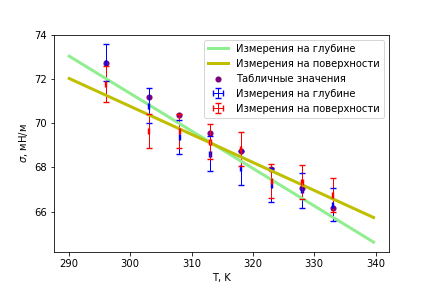
\includegraphics[width=\textwidth]{sigma}
\end{center}
\caption{Зависимость коэффицента поверхностного натяжения воды от температуры} \label{sigma}
\end{figure}
Значения коэффицента натяжения при измерениях на глубине сосуда близки к табличным, их и будем учитывать при дальнейших расчетах. Несовпадение с результами измерений на поверхности жидкости объясняется теплопроводностью металла. 

Из аппроксимации графика найдем $\frac{d\sigma}{dt}$:

\begin{table}[h!]
\caption{Зависимость коэффицента поверхностного натяжения воды от температуры}
\label{dsigma}
\begin{tabular}{|l|l|l|}
\hline
$\frac{d\sigma}{dt}$, $10^{-3}\; \frac{мН}{м\cdot K}$ & $\sigma_\sigma$, $10^{-3}\; \frac{мН}{м\cdot K}$ & $\varepsilon$, \%\\ \hline
-0.17         & 0.02                  & 9.6       \\ \hline
\end{tabular}
\end{table}

Используя полученные результаты, построим графики зависимости:

1. теплоты образования единицы поверхности жидкости $q = -T\cdot \frac{d\sigma}{dt}$ (рис. \ref{q})

2. поверхностной энергии $U$ единицы площади $F$:  $U/F = (\sigma -T\cdot  \frac{d\sigma}{dt})$ (рис. \ref{U/F}). График выглядит как случайно разбросанные точки, однако его аппроксимация близка к горизонтали, что подтвреждается теорией. Разброс точек возникает из-за неидеальности полученных значений.

\begin{figure}[h!]
\begin{center}
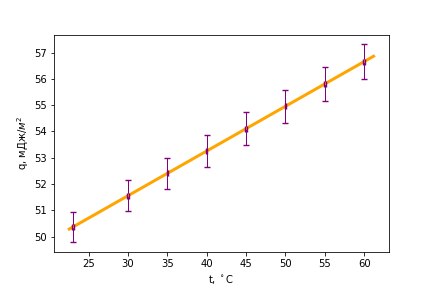
\includegraphics[width=0.95\textwidth]{q}
\end{center}
\caption{Зависимость теплоты образования единицы поверхности жидкости от температуры} \label{q}
\end{figure}

\begin{figure}[h!]
\begin{center}
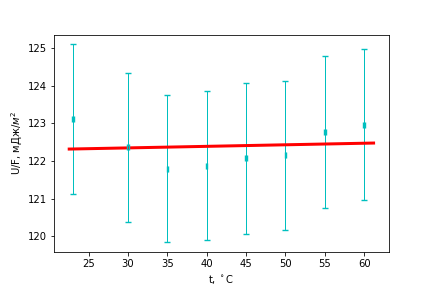
\includegraphics[width=0.95\textwidth]{U}
\end{center}
\caption{Зависимость поверхностной энергии единицы площади от температуры} \label{U/F}
\end{figure}

\section{Выводы}
\hspace{5mm}
1. Измерены коэффциенты поверхностного натяжения при разных температур, пронаблюдалась близость полученных результатов к табличным значениям.
 
2. Получена температурная зависимость коэффициента поверхностного натяжения воды от температуры. $\frac{d\sigma}{dt} \;=\; -0.17 \pm 0.02$, $10^{-3}\; \frac{мН}{м\cdot K}$ при теоретическом значении $\frac{d\sigma}{dt} = -0.15$, $10^{-3}\; \frac{мН}{м\cdot K}$

3. Вычислены зависимости теплоты образования единицы поверхности жидкости от температуры и поверхностной энергии единицы площади от температуры, постоянство второй из них подтверждается теоретически.
\end{document}